\chapter{Relevant Concepts}
\label{sec:concepts}
\ifpdf
    \graphicspath{{3_concepts/figures/PNG/}{3_concepts/figures/PDF/}{3_concepts/figures/}}
\else
    \graphicspath{{3_concepts/figures/EPS/}{3_concepts/figures/}}
\fi


Point clouds are collections of points in space that represent geometric shapes in their simplest forms, so data structures they are a set of unordered vectors of points \cite{10.1145/3326362}. PointNet expects its input points from Euclidean Space, hence this section addresses key concepts pertaining to point sets in $\mathbb{R}^n$. Understanding the properties of point sets is essential in order to understand the suitability of KM3NeT data and the rationale behind data preparation. This section also discusses key concepts underlying PointNet architecture. 

\section{Properties of Input Point Sets}
\label{sec:concepts-pointset}
Qi et al. (2017) identified three main properties that input point sets must follow.  
 
\begin{enumerate}
    \item \textbf{Unordered}: Point sets are unordered and so 3D input data accordingly must be invariant to $N!$ permutations in the order that it is provided to the network.
    \item \textbf{Interaction among points}: Point sets originating from a space with a distance metric demonstrates meaningful relationship amongst neighbouring points. This will allow PointNet to capture and learn local and global structures.
    \item \textbf{Invariant under transformations}: Unordered point sets should be invariant to transformations. Learned representations such as rotation or translation of input data should remain unaffected by the applied transformations in terms of global structures \cite{qi2017pointnet}. 
\end{enumerate}


\section{PointNet Architecture}
According to Qi et al. (2017), PointNet can perform both classification and segmentation tasks. This thesis only focuses on the classification network due to its relevance to the research problem. Figure \ref{fig:pointnet-architecture} shows an overview of the PointNet architecture. The classification network accepts \texttt{n} points as input and applies input and feature transformations. A shared multi-layer perceptron (MLP) is used to map points from the \texttt{x, y, z} dimensions to 64 dimensions. This step is duplicated to then map points from 64 dimensions to 1024 dimensions. Next, point features are aggregated though \textit{max pooling} to generate a global features vector in $\mathbb{R}^{1024}$. Max pooling is a technique that is used to down-sample input via sample discretization to a more abstract output \cite{ian2016deep}. Finally, a MLP is used to map global feature vector to \textit{k} classification scores \cite{qi2017pointnet}. 

\begin{figure}[ht!]
    \centering
    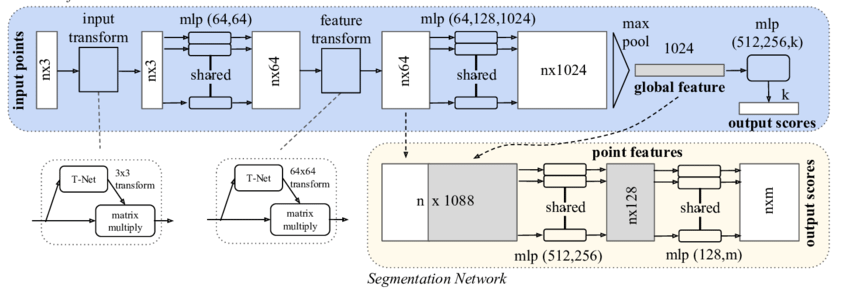
\includegraphics[width=\linewidth]{pointnet_architecture.png}
    \caption{PointNet Architecture for Classification and Segmentation \cite{qi2017pointnet}.
    \textit{mlp} indicates multi-layer perceptron; numbers in brackets are the layer sizes.}
    \label{fig:pointnet-architecture}
\end{figure}

Feature and input transformations are significant to the architecture, and is additionally described under permutation and transformation invariance. 

\subsection{Permutation Invariance}
Point clouds are unstructured, numerical sets and invariant to permutations ie., for $N$ points, there are $N!$ valid permutations (section \ref{sec:concepts-pointset}). Symmetric functions are therefore used to make PointNet invariant to input permutations \cite{qi2017pointnet}. Specifically, max pooling is used when \texttt{n} input points are mapped to higher dimensional space and then used directly for classification \cite{qi2017pointnet}. This can be seen in Figure \ref{fig:pointnet-symmetric}

\begin{figure} [ht!]
    \centering
    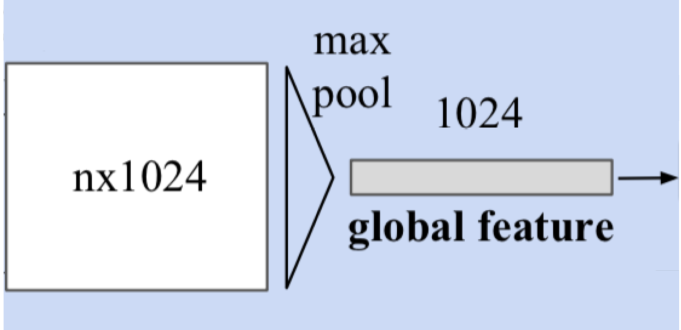
\includegraphics[width=0.5\linewidth, height=3cm,keepaspectratio]{symmetric_function.png}
    \caption{Symmetric Function with Max Pool Applied to Global Features \cite{qi2017pointnet}}
    \label{fig:pointnet-symmetric}
\end{figure}

\subsection{Transformation Invariance}
Point clouds must be invariant to certain geometric transformations (section \ref{sec:concepts-pointset}). If point clouds undergo transformation, then it is necessary that the classification labelling must be invariant as well. To ensure that this is the case, input and feature transformation sub-networks are used to provide normalisation to objects. \textit{T-Net} - a regression network is tasked with predicting a $n{\times}n$ transformation matrix.  

\begin{figure}[ht]   
\centering
\subfloat[Input Transformation]{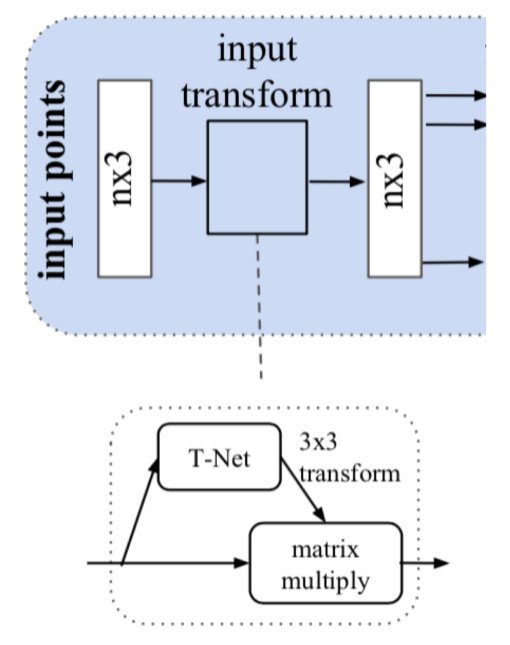
\includegraphics[width=0.4\textwidth, height=5.1cm,keepaspectratio]{input_transform.png}\label{fig:input_transform}}
\subfloat[Feature Transformation]{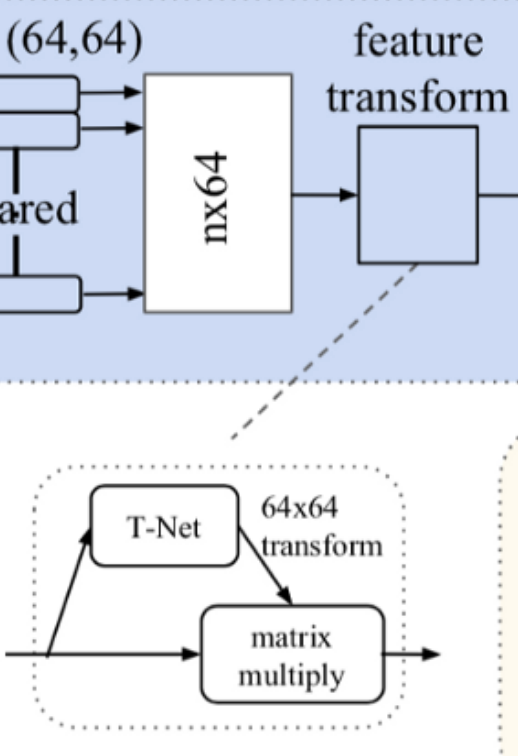
\includegraphics[width=0.4\textwidth,
height=5cm,keepaspectratio]{feature_transform.png}\label{fig:feature_transform}}
\caption[]{Input and Feature Transforms within PointNet}
\label{fig:input_feature_transform}
\end{figure}

For input transformations, \textit{n} input points are represented as a vector and  mapped to the embedding spaces. Geometric transformation then becomes easy to apply and involves matrix multiplying each point with a transformation matrix. Here, the T-Net predicts a $3{\times}3$ transformation matrix, which is then matrix multiplied with the $n{\times}3$ input (Figure \ref{fig:input_feature_transform}).

For feature transformation of the 64-dimensional embedding space, the corresponding T-Net predicts a $64{\times}64$ transformation matrix (Figure \ref{fig:input_feature_transform}). The increased number of trainable parameters leads to the potential for overfitting and instability during training, so a regularisation term is added to the loss function to constrain the feature matrix to be close to the orthogonal matrix:

\begin{equation}
    \mathcal{L}_{reg} = || I - AA^{T} ||^{2}_{F}
\end{equation}

where \textit{A} is the matrix predicted by the T-Net. 

So, PointNet is capable of learning from unordered, raw point clouds as long as the properties of point sets are maintained. This is relevant to the thesis and validated when preparing training data. Additional transformation functions within the network further ensure that the data respects invariance to permutations and transformations. These concepts are used by this thesis in the upcoming pipeline to ensure absolute accordance with rules governing point sets. 
